\section{Information about this thesis}

This thesis, including this document, is contained in a single git repository
that can be found at GitHub\autocite{git-repo}.

All the work that has been done is open sourced under the Apache License 2.0,
except the Go source code, which has its own license.

To view the code, build or reproduce results, this git repository can be cloned
and its submodules checked out. The version that has been submitted can be checked
out through the tag `v1.0.0':
\begin{bashcode}
$> git clone https://github.com/tommyknows/bachelor-thesis.git
$> cd bachelor-thesis
$> git checkout v1.0.0
$> git submodule init
$> git submodule update
\end{bashcode}

The directory `thesis' contains the \LaTeX\ code for this paper. There is a helper
required for displaying code in the thesis which is located in `thesis/utils' and
needs to be built with `go build .'. However, a PDF which should be on the same state
as the source is provided in the repository too (`thesis/thesis.pdf').

The `work' directory contains code that has been developed in this thesis. In this
directory, the Go and funcheck source code can be found (see Appendix~\ref{appendix:install-fgo}
and~\ref{appendix:build-funcheck}). Further, some examples
of functional Go have been developed in the `example' directory. The `common-list-functions'
folder contains the script as mentioned in Appendix~\ref{appendix:function-occurrences}.

\section{Example for Functional Options}\label{appendix:funcopts}

This source code example demonstrates `functional options' as introduced in this paper.
Functional options are usually passed to a constructor to configure the new instance, in
this case a web server. The advantages of functional options are that the API ends up to
be cleaner and more easily extensible and allows the default use-case to be as simple
as possible.

\begin{code}
    \gofile{../work/examples/functional-options/main.go}%
    \caption{Functional Options for a simple web server}
\end{code}

\section{Analysis of function occurrences in Haskell code}\label{appendix:function-occurrences}
The results of the analysis have been acquired by running the `count-function' script
that is located in `work/common-list-functions' in the git repository\autocite{git-repo}.

The script utilises \href{https://github.com/BurntSushi/ripgrep}{ripgrep} to count the number of occurrences, so
this must be installed in order to run this script.

\begin{bashcode}
./count-function.sh ":" "((map)|(fmap))" "((foldr)|(foldl'?))" "filter" "reverse" "take" "drop" "sum" "zip" "product" "maximum" "min
imum"
Searching for occurrences in subdirectories of ./common-list-functions
Found 2912 occurrences of ":"
Found 1873 occurrences of "((map)|(fmap))"
Found 303 occurrences of "((foldr)|(foldl'?))"
Found 262 occurrences of "filter"
Found 154 occurrences of "reverse"
Found 108 occurrences of "take"
Found 81 occurrences of "drop"
Found 44 occurrences of "sum"
Found 38 occurrences of "zip"
Found 15 occurrences of "product"
Found 45 occurrences of "maximum"
Found 10 occurrences of "minimum"
\end{bashcode}

The terms are searched with a leading and trailing space to get exact matches. Further, as can be seen in
the call to the script, the search combines the results of map together with fmap, and foldr with foldl
and foldl'.

\section{Mutating variables in Go}\label{appendix:mutation}

Source Code~\ref{code:mutation} shows how pointers are used to mutate data in Go. This does
not necessarily need to be a `struct' type, pointers can be used of any type.
Pointers have to be used to modify values because Go is a copy-by-value language and thus
copies the parameters that are passed to a function.

\begin{code}
	\gofile{../work/examples/mutate/main.go}%
	\caption{Example on how to mutate data in Go}\label{code:mutation}
\end{code}

\section{Shadowing variables in Go}\label{appendix:shadowing}

Source Code~\ref{code:shadowing} demonstrates the block scoping and shadowing rules
in Go.

\begin{code}
	\gofile{../work/examples/shadowing/main.go}%
	\caption{Example on how shadowing works on block scopes}\label{code:shadowing}
\end{code}

\section{Foldl and Foldl' difference}\label{appendix:foldl-strictness}

This code example shows the difference between foldl and foldl' in their
execution. What can be seen is that foldl builds up a call stack, while
foldl' executes the calls during the traversal.

\begin{code}
    \begin{haskellcode}
> (?) :: Int -> Int -> Int
> _ ? 0 = 0
> x ? y = x*y
>
> list :: [Int]
> list = [2,3,undefined,5,0]
>
> foldl (?) 1 list
foldl (?) 1 [2,3,undefined,5,0] -->
foldl (?) (1 ? 2) [3,undefined,5,0] -->
foldl (?) ((1 ? 2) ? 3) [undefined,5,0] -->
foldl (?) (((1 ? 2) ? 3) ? undefined) [5,0] -->
foldl (?) ((((1 ? 2) ? 3) ? undefined) ? 5) [0] -->
foldl (?) (((((1 ? 2) ? 3) ? undefined) ? 5) ? 0) [] -->
((((1 ? 2) ? 3) ? undefined) ? 5) ? 0 -->
0

> foldl' (?) 1 list
foldl' (?) 1 [2,3,undefined,5,0] -->
    1 ? 2 --> 2
foldl' (?) 2 [3,undefined,5,0] -->
    2 ? 3 --> 6
foldl' (?) 6 [undefined,5,0] -->
    6 ? undefined -->
*** Exception: Prelude.undefined
    \end{haskellcode}
    \caption{foldl and foldl' strictness\autocite{fold-types}}
\end{code}

\section{Workaround for the missing foldl implementation in Go}\label{appendix:foldl-go}

This code block exemplifies how foldl could be implemented in Go code. It is based on the example
from Appendix~\ref{appendix:foldl-strictness}, rewritten in Go. While Go does not know about
the concept of laziness, the programmer may implement the laziness himself by working with function
closures.

In this example, \mintinline{go}|*int| is used instead of \mintinline{go}|int| to simulate Haskell's
\mintinline{haskell}|undefined| with a nil-pointer.
If a nil-pointer is dereferenced, the program will panic.

In the lazy version of this code (utilising `myFold' and `mulLazy'), the panic does not occur because
the nil-pointer is never dereferenced as the function closure is never executed. This is equal
to the `foldl' demonstration in Appendix~\ref{appendix:foldl-strictness}.

The non-lazy version (`foldl' and `mul') executes the function while traversing the slice and thus panics.

\begin{code}
	\gofile{../work/examples/foldl-workaround/main.go}%
	\begin{bashcode}
$> fgo run .
0
panic: runtime error: invalid memory address or nil pointer dereference
[signal SIGSEGV: segmentation violation code=0x1 addr=0x0 pc=0x109e945]

goroutine 1 [running]:
...
	\end{bashcode}
	\caption{Working around the missing foldl implementation in Go\label{code:foldl-go}}
\end{code}

\section{Prettyprint implementation}\label{appendix:prettyprint-func}

These code blocks show the same package `prettyprint', once in idiomatic Go and once
in functional Go. What can be seen is that the \mintinline{go}|for| loops have been replaced
by the usage of `foldl' and anonymous functions.

\begin{code}
	\gofile{../work/funcheck/prettyprint/prettyprint.go}%
	\caption{The original prettyprint implementation\autocite{prettyprint-orig}}
\end{code}
\begin{code}
	\begin{gocode}
package prettyprint

import (
	"bytes"
	"fmt"
	"go/ast"
	"go/printer"
	"go/token"

	"golang.org/x/tools/go/analysis"
)

var Analyzer = &analysis.Analyzer{
	Name: "prettyprint",
	Doc:  "prints positions",
	Run:  run,
}

type null struct{}

func checkDecl(as *ast.DeclStmt, fset *token.FileSet) {
	fmt.Printf("Declaration %q: %v\n", render(fset, as), as.Pos())

	check := func(_ null, spec ast.Spec) (n null) {
		val, ok := spec.(*ast.ValueSpec)
		if !ok {
			return
		}
		if val.Values != nil {
			return
		}
		if _, ok := val.Type.(*ast.FuncType); !ok {
			return
		}
		fmt.Printf("\tIdent %q: %v\n", render(fset, val), val.Names[0].Pos())
		return
	}

	if decl, ok := as.Decl.(*ast.GenDecl); ok {
		_ = foldl(check, null{}, decl.Specs)
	}
}

func checkAssign(as *ast.AssignStmt, fset *token.FileSet) {
	fmt.Printf("Assignment %q: %v\n", render(fset, as), as.Pos())

	check := func(_ null, expr ast.Expr) (n null) {
		ident, ok := expr.(*ast.Ident) // Lhs always is an "IdentifierList"
		if !ok {
			return
		}

		fmt.Printf("\tIdent %q: %v\n", ident.String(), ident.Pos())

		switch {
		case ident.Name == "_":
			fmt.Printf("\t\tBlank Identifier!\n")
		case ident.Obj == nil:
			fmt.Printf("\t\tDecl is not in the same file!\n")
		default:
			// make sure the declaration has a Pos func and get it
			declPos := ident.Obj.Decl.(ast.Node).Pos()
			fmt.Printf("\t\tDecl %q: %v\n", render(fset, ident.Obj.Decl), declPos)
		}

		return
	}
	_ = foldl(check, null{}, as.Lhs)
}

func run(pass *analysis.Pass) (interface{}, error) {
	inspect := func(_ null, file *ast.File) (n null) {
		ast.Inspect(file, func(n ast.Node) bool {
			switch as := n.(type) {
			case *ast.DeclStmt:
				checkDecl(as, pass.Fset)
			case *ast.AssignStmt:
				checkAssign(as, pass.Fset)
			}
			return true
		})
		return
	}
	_ = foldl(inspect, null{}, pass.Files)

	return nil, nil
}

// render returns the pretty-print of the given node
func render(fset *token.FileSet, x interface{}) string {
	var buf bytes.Buffer
	if err := printer.Fprint(&buf, fset, x); err != nil {
		panic(err)
	}
	return buf.String()
}
	\end{gocode}
	\caption{The refactored, functional prettyprint implementation\autocite{prettyprint-functional}}
\end{code}

\section{Imitating Sum types in Go}\label{appendix:sum-types}

\begin{code}
    \gofile{../work/examples/sumtypes/main.go}%
\caption{Demonstration of how sum types can be imitated with interfaces}
\end{code}

\section{Compiling and using functional Go}\label{appendix:install-fgo}

To compile and use the changes to the Go compiler that have been implemented in
this thesis, these instructions should be followed.

First, check out the Go source code:

\begin{bashcode}
$> git clone https://github.com/tommyknows/go.git && cd go
$> git checkout bachelor-thesis
\end{bashcode}

\subsection{With Docker}

If Docker is installed on your system, you can follow these steps from within
the checked out `go' git repository on the branch `bachelor-thesis'.
The downside of this approach is that it complicates building and sharing binaries.
To compile your own project, the directory has to be mounted into the container.
If your Guest OS is not Linux, cross-compilation is required so that the executable
can be ran on the host.

These steps have been wrapped inside a script that prints out the necessary commands
to configure your environment.

\begin{bashcode}
$> eval "$(./setup-docker.sh)"
\end{bashcode}
The commands within the shell script will
build Go in the container and print commands to configure the environment. The `eval'
command then executes these printed commands. Executing this command may take a while,
as the Go compiler is compiled within this process.

To build projects with the functional Go installation, simply use `fgo' on the command line.
An alias has been created that mounts the current directory and executes the `fgo'
command within the container.

Note that if this only configures the `fgo' command in the current shell session. To
persist it across shell-sessions, execute the script without eval:
\begin{bashcode}
$> ./setup-docker.sh
\end{bashcode}

And add the printed commands to your `.bashrc' (or equivalent). Further, you may
also need to change the binary path from `/tmp/fgo/bin' to a path which is not
cleaned up regularly.

\subsection{With a working Go installation}

If you already have a working Go installation on your system, the following
steps provide a way to get functional Go up and running in the same way
a normal go installation does.

These steps need to be executed from within the checked out `go' git
repository on the branch `bachelor-thesis'.

Build the functional Go binary and configure the environment:
\begin{bashcode}
$> cd ./src
$> ./make.bash
$> ln -s $(realpath $(pwd)/../bin/go) /usr/local/bin/fgo
$> go env -w GOROOT=$(realpath $(pwd)/..)
\end{bashcode}

The `go env' command sets the GOROOT to point to the newly compiled tools
and source code and is valid for the current shell session only.

\subsection{Using the installation}

After these steps, the binary (or alias) `fgo' can be used to test and build
functional Go code. `fgo' is not different to the normal `go' command, so
all commands that work with the normal `go' command also work with
the `fgo' command.

\begin{bashcode}
$> cd <code directory>
$> fgo test ./...
$> fgo build ./...
\end{bashcode}


\section{Building Funcheck}\label{appendix:build-funcheck}

Funcheck needs to be built against functional Go to properly detect the builtin functions.
If you have not done so already, install `fgo' as shown in Appendix~\ref{appendix:install-fgo}.

Then, funcheck can be installed directly with `go get' (or rather, `fgo get'). `go get'
downloads the source code to the Go modules directory (usually in \mintinline{bash}|$GOPATH/pkg/mod|),
compiles the specified package and moves the binary to \mintinline{bash}|$GOPATH/bin|.

\begin{bashcode}
$> # go get should not be called from within a go module
$> cd /tmp
$> fgo get github.com/tommyknows/funcheck
$> funcheck -h
\end{bashcode}

This installs `funcheck' into \mintinline{bash}|$GOBIN| or, if \mintinline{bash}|$GOBIN|
is not set, into \mintinline{bash}|$GOPATH/bin|.

You can also clone the git repository and use `fgo build' to build `funcheck':
\begin{bashcode}
$> git clone https://github.com/tommyknows/funcheck.git
$> cd funcheck
$> fgo build .
$> mv ./funcheck /usr/local/bin/funcheck
$> funcheck -h
\end{bashcode}

To run funcheck against the current directory / package, simply run
\begin{bashcode}
$> funcheck .
\end{bashcode}

\section{Building Gopls}\label{appendix:build-gopls}

Gopls is the official language server for Go. Similar to funcheck, there are two options
to install it on your local machine.

Installing with `go get':
\begin{bashcode}
$> # go get should not be called from within a go module
$> cd /tmp
$> fgo get golang.org/x/tools/gopls
$> gopls -h
\end{bashcode}

Or by downloading the source manually:
\begin{bashcode}
$> git clone https://github.com/golang/tools.git
$> cd ./tools/gopls
$> fgo build .
$> mv ./gopls /usr/local/bin/gopls
$> gopls -h
\end{bashcode}

% generate a chapter without the chapter heading
\clearpage
\phantomsection
\addtocounter{section}{1}
\addcontentsline{toc}{section}{%
	\protect\numberline{\thesection}%
	Assignment}
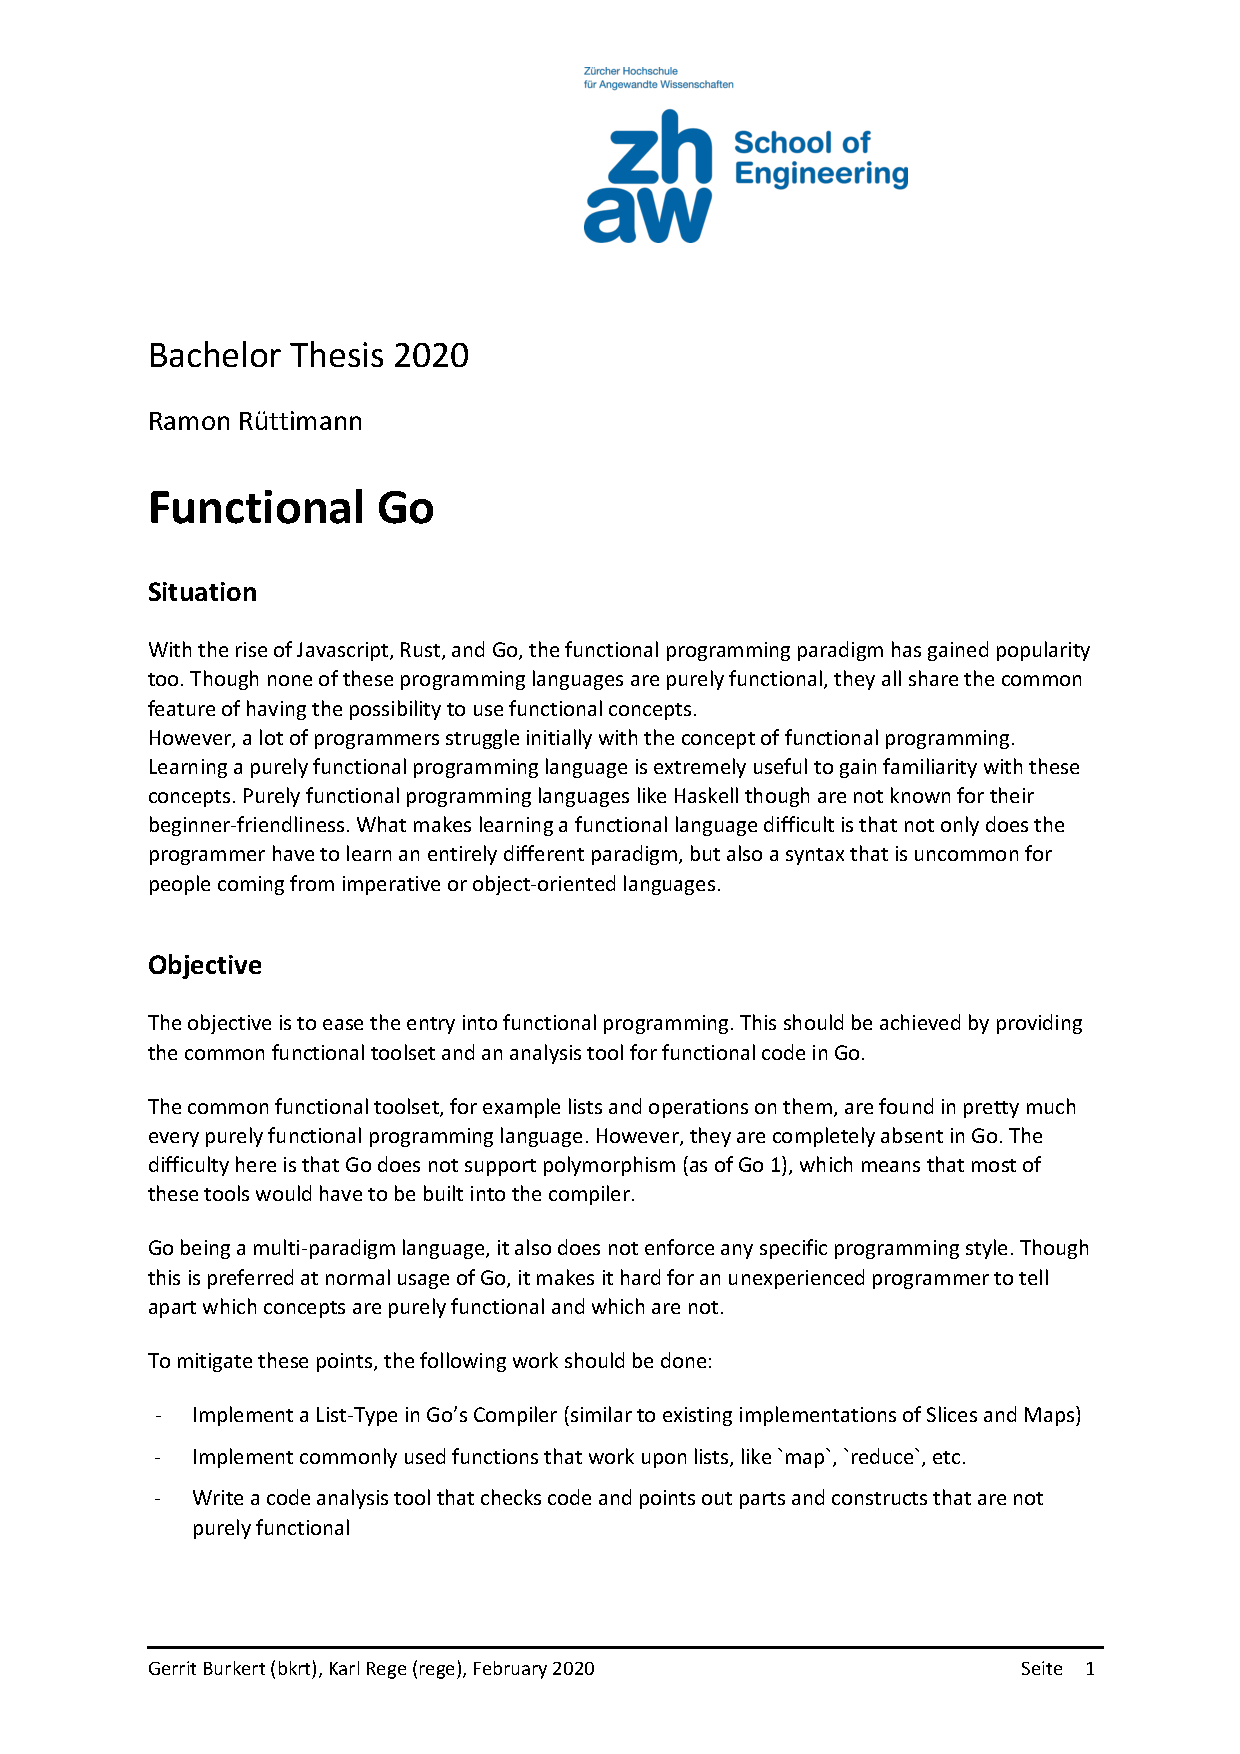
\includepdf[pages=-]{assignment.pdf}
